\RequirePackage{fix-cm}
%
%\documentclass{svjour3}                     % onecolumn (standard format)
%\documentclass[smallcondensed]{svjour3}     % onecolumn (ditto)
\documentclass[smallextended]{svjour3}       % onecolumn (second format)
%\documentclass[twocolumn]{svjour3}          % twocolumn

\smartqed  % flush right qed marks, e.g. at end of proof

\usepackage{graphicx}
\usepackage{algorithm}
\usepackage{algorithmic}
\journalname{Automated Software Engineering}

\begin{document}

\title{Empirically Evaluating the Efficiency of Search-based Test Data
Generation for Relational Database Schemas}

%\subtitle{Do you have a subtitle?\\ If so, write it here}

%\titlerunning{Short form of title}        % if too long for running head

\author{Cody Kinneer         \and
        Luke Smith \and
        Gregory Kapfhammer \and
        Chris Wright \and
        Phil McMinn
}

%\authorrunning{Short form of author list} % if too long for running head

\institute{F. Author \at
              first address \\
              Tel.: +123-45-678910\\
              Fax: +123-45-678910\\
              \email{fauthor@example.com}           %  \\
%             \emph{Present address:} of F. Author  %  if needed
           \and
           S. Author \at
              second address
}

\date{Received: date / Accepted: date}
% The correct dates will be entered by the editor


\maketitle

\begin{abstract}
When evaluating an algorithm, it is often useful to speak of it's
efficiency in terms of it's worst case complexity.  However, for certain
cases such as search-based algorithms, determining an algorithm's
efficiency by theoretical analysis is difficult, and has not been
reported in the literature. This paper introduces a
framework for conducting automated empirical studies of algorithms by
doubling the size of the input and observing the change in execution
time. We apply this method to the domain of data generation for
relational database schemas.  After implementing a technique for 
systematically doubling the size of schemas, we conduct an
empirical study on the search-based data generation tool
\textit{SchemaAnalyst}. For the parameters of \textit{SchemaAnalyst}
studied, the study concludes that \textit{SchemaAnalyst} is $O(n^2)$
with respect to the number of check constraints in the input schema.


\keywords{First keyword \and Second keyword \and More}
% \PACS{PACS code1 \and PACS code2 \and more}
% \subclass{MSC code1 \and MSC code2 \and more}
\end{abstract}

\section{Introduction}
Search-based algorithms allow the application of guidance to problems.
The algorithm attempts to improve a potential solution until the
solution is acceptable. Without the use of a search-based strategy, a
problem might be approached with a random sampling or greedy
technique. In the
domain of data generation for software testing, this means that rather
than randomly selecting inputs from a program's input space, the data
generator can actively seek out qualities of an input that best fulfill the test's goals \cite{McMinn:Thesis}. While this
technique has been applied to various problems, including test suite
prioritization \cite{Walcott:tsp} and testing
relational database schemas \cite{Kapfhammer2013}, 
as far as we know, no research has been done on evaluating the efficiency
of search-based test data generation. 

This paper presents an empirical study of the search-based data
generation tool, called \textit{SchemaAnalyst}, which generates test suites for
relational database schemas.  To evaluate \textit{SchemaAnalyst}, a tool
was implemented in Java to systematically double the size of the
program's input and record the change in it's execution time. Using this
technique, for the coverage criterion and data generator tested, 
\textit{SchemaAnalyst} was found to be $O(n^2)$ with respect
to the number of check constraints in the schema. The contributions of
this paper are therefore as follows:
\begin{enumerate}
  \item A framework for automated doubling experiments
  \item An empirical study evaluating the efficiency of a search-based
    data generation tool
  \end{enumerate}

\section{Background}

Worst-case time complexity is a useful measure of an algorithms
efficiency, or how increasing the size
of the input $n$ increases the execution time of the algorithm, $f(n)$.
This relationship is often expressed in big-Oh notation, where $f(n)$
is $O(g(n))$ means that the time increases by order of $g(n)$. The
worst-case complexity of an algorithm is evident when $n$ is large 
\cite{Goodrich:Data}. One approach for determining the big-Oh complexity
of an algorithm is to conduct a doubling experiment. By measuring the
time needed to run the algorithm on an input $n$, and the time needed to
run on $2n$, the order of growth of the algorithm can be determined \cite{Mcgeoch:Algorithmics,
Sedgewick:Analysis}. 

Intuitively, the goal of a doubling experiment is to draw a conclusion
regarding the efficiency of the algorithm from the ratio
$f(2n)/f(n)$. This ratio represents the factor of change in runtime from
input $n$ to $2n$. A ratio of $2$ would indicate that doubling the
input resulted in runtime doubling. We could then conclude that the
algorithm under study is $O(n)$. 

\section{Technique}
To determine worst case complexity, an input $n$ is doubled until the 
ratio $f(2n) / f(n)$ converges to a stable value. To account for random
error, every time $n$ is doubled, $f(n)$ is recorded ten times
, and the median time is used for calculating the ratios.  We chose
median to minimize the effect of outliers. If mean is used instead, a
single abnormally long run could have a large effect on the result. The overall 
structure of the experiment is shown in Algorithm~\ref{alg:main}.

This convergence checking is necessary because of the fact that worst-case
time is only apparent for large values of $n$. If too few doubles
are tried, then the experiment may terminate before $n$ reaches a value
where the true worst-case time complexity is apparent. At the same time,
for inefficient  algorithms, each additional double run incurs a substantial
time overhead. To conduct the testing efficiently, the experiment should
terminate as quickly as possible.

To test for convergence, the last four ratios are compared, and the
sum of differences between them is compared to a tolerance value. A
tolerance value of $0.40$ was chosen  by performing doubling
experiments on various algorithms with known worst case time
complexities, and observing that the ratio converged to the correct
value when $\mathit{diff} < 0.40$. The convergence algorithm is shown
as Algorithm~\ref{alg:convergence}.
  
Another consequence of worst-case time only being apparent for large
$n$, is that a very small initial $n$ may appear to converge to $1$,
which indicates constant time. To prevent the
experiment from incorrectly terminating given a small starting $n$, we
require that a program under study display a ratio of $1$ for many
runs before judging that the ratio does in fact converge to $1$. In this case,
the experiment is considered convergent if the ratio remains $1$ for 
twenty consecutive doubles.  Because $1$ signifies constant or logarithmic 
time, requiring these doubles does not significantly increase the time needed
to run the experiment, while providing assurance that a small ratio is not due
to an insufficiently small $n$. This  is shown as 
Algorithm~\ref{alg:tuning}.

\begin{algorithm}[t]
    \caption{Run Doubling Experiment}
    \begin{algorithmic}
      \WHILE{Diff not convergent || N not large enough}
        \FOR{$\mathit{count} < 10$}
        \STATE Run Test
        \STATE $\mathit{count}++$
        \ENDFOR
        \STATE Double Schema
        \ENDWHILE
    \end{algorithmic}
    \label{alg:main}
  \end{algorithm}

 \begin{algorithm}[t]
    \caption{Diff not Convergent}
    \begin{algorithmic}
      \STATE $\mathit{diff} = |(r_4 - r_3) + (r_3 -r_2) + (r_2 - r_1)|$
      \IF{$\mathit{diff} < 0.40$}
      \RETURN FALSE
      \ELSE
      \RETURN TRUE
      \ENDIF
    \end{algorithmic}
    \label{alg:convergence}
  \end{algorithm}

 \begin{algorithm}[t]
    \caption{N not Large Enough}
    \begin{algorithmic}
      \IF{$\mathit{ratio} \approx 1$}
      \IF{$\mathit{Doubles} < 20$}
      \STATE minRuns++
      \RETURN TRUE
      \ENDIF
      \ENDIF
      \RETURN FALSE
    \end{algorithmic}
    \label{alg:tuning}
  \end{algorithm}

\section{Experimental Design}
To analyze \textit{SchemaAnalyst}, the iTrust and NistWeather case
studies provided by \textit{SchemaAnalyst} were used as the initial 
input schemas.
Both of these schemas are taken from real world applications. The factor $n$
under study was the number of check constraints present on the schema.  
A Java program was
implemented to double the number of these constraints. Generating
synthetic check constraints is non-trivial because there are many
possible check constraints, and generating a constraint that is
unsatisfiable might cause the data generation tool to take a longer
amount of time than should be the case. To avoid this problem, we
instead duplicate the existing check constraints present on the schema
rather than attempt to generate new ones. This technique is easy
to implement and ensures that the check constraints added are
semantically valid.  For every table in the input schema, the tool 
duplicated the existing check constraints and added the duplicates 
to the table.  

The test suite generation tool provided by \textit{SchemaAnalyst}
requires a coverage criterion and a data generator to be specified. A
coverage criterion is a system of rules that generate test requirements
\cite{Ammann:Testing}. The data generator is the object that generates
the test data according to the rules specified by the coverage
criterion. The criterion used in the experiment was
\textsc{constraintCACCoverage}, 
the data generator was \textsc{directedRandom}. The
doubling experimentation software were implemented in Java, and were both compiled and run using
version 1.7 of the compiler and Java Virtual Machine. The experiment was executed on an Ubuntu 13.10 machine with a 2.4
GHz quad core CPU running the 3.11.0-18-generic x86\_64 GNU/Linux
kernel and 4G.

\section{Results}
Our technique was able to determine the worst-case time
complexity of \textit{SchemaAnalyst} with regard to the number of check
constraints on the input schema, using the
\textsc{constraintCACCoverage} coverage criterion and the
\textsc{directedRandom} data generator. Under these conditions, 
\textit{SchemaAnalyst} displayed $O(n^2)$ behavior. Figures~\ref{fig:iTrust} 
and~\ref{fig:NistWeather} show the data collected during the experiment with a
quadratic fit. The horizontal axis shows by what factor the number of initial
check constraints $i$ have been increased. For $x = 100$, the number of check
constraints on the schema is $100i$. The vertical axis shows the time in
nanoseconds \textit{SchemaAnalyst} needed to generate a test suite for
the input schema. Each point on the graph represents the amount of time
\textit{SchemaAnalyst} ran for a schema with $ix$ check constraints.
The equation shown is the best fit quadratic equation for that data.  A
quadratic relationship indicates that \textit{SchemaAnalyst} is
$O(n^2)$.  The value $r^2$ is a measure of the quality of fit between a model and
the data. The closer $r^2$ is to $1$, the better the quality of the
model.  An $r^2$ of $.997$ and $1$ indicates that the models are a good fit for
the data.

\begin{figure*}
\centering
  \centering
  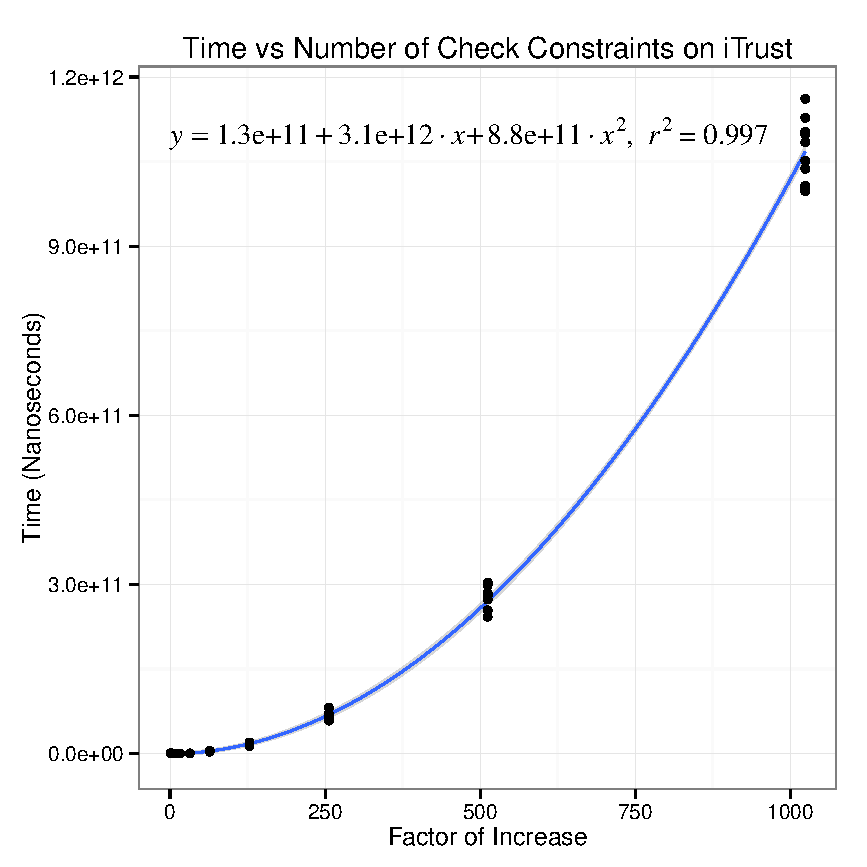
\includegraphics[width=.5\linewidth]{iTrustChecks.pdf}
  \caption{Time vs Check Constraints on iTrust.}
  \label{fig:iTrust}
\end{figure*}
\begin{figure*}
  \centering
  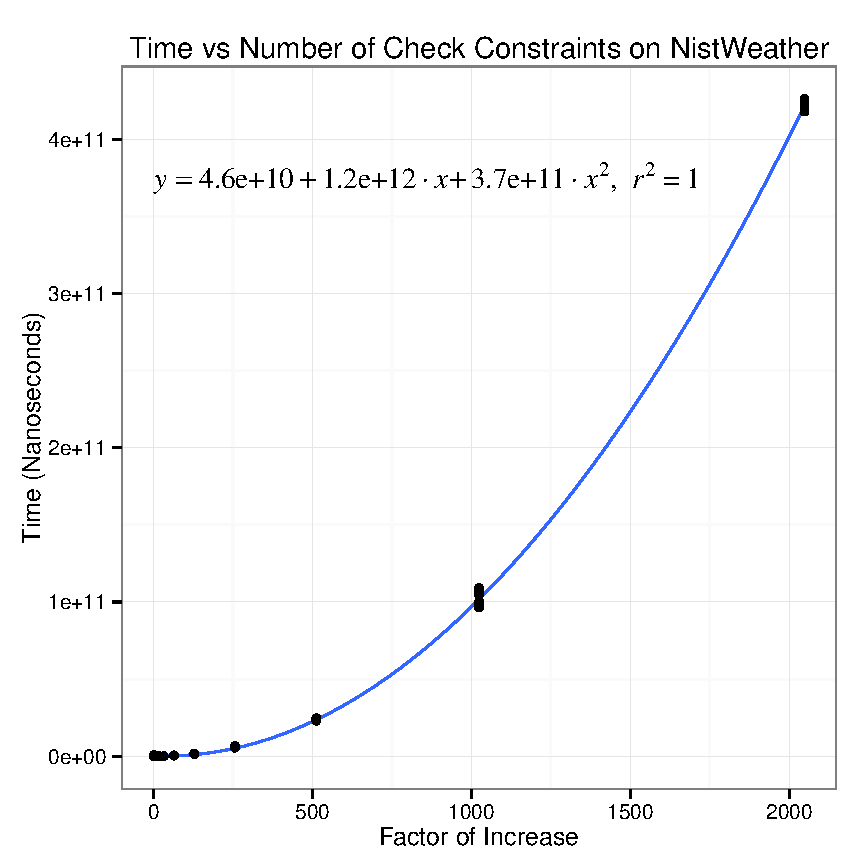
\includegraphics[width=.5\linewidth]{NistWeatherChecks.pdf}
  \caption{Time vs Check Constraints on NistWeather.}
  \label{fig:NistWeather}
\end{figure*}

\subsection*{Threats to Validity}
Our technique for doubling the number of check constraints on the schema
is simply to duplicate the existing check constraints. It is possible
that \textit{SchemaAnalyst} does less work processing these copied check
constraints than it would given unique check constraints. However,
doubling the check constraints in this way is an easy to implement,
semantically significant way of evaluating \textit{SchemaAnalyst}.

Additionally, since worst-case time is only apparent for large $n$, 
it is possible that the experiment terminated too quickly.  To guard 
against this problem, Algorithms~\ref{alg:convergence} and ~\ref{alg:tuning}
were tested on various other algorithms with known worst-case complexities, and 
found to be reliable.

\section{Conclusions and Future Work}
The automated doubling experiment was able to determine the worst case
time complexity of \textit{SchemaAnalyst} with respect to the number of
check constraints in the input schema, for the
\textsc{constraintCACCoverage} criterion and the
\textsc{directedRandom} data generator.  Additional experiments will be
conducted on other criterions and data generators. Additionally, other factors 
that may influence the runtime of schema analysis,
such as the number of primary keys, foreign keys, tables, columns, etc
will be investigated.


% BibTeX users please use one of
\bibliographystyle{spbasic}      % basic style, author-year citations
%\bibliographystyle{spmpsci}      % mathematics and physical sciences
%\bibliographystyle{spphys}       % APS-like style for physics
\bibliography{sigproc}   % name your BibTeX data base

\end{document}
